\section{Simple Machines}

%$\textbf{Mechanical Advantage (M.A.)} = \text{Load} \div \text{Effort}$\\
%$\textbf{Velocity Ratio (V.R.)} = \text{effort distance} \div \text{load distance}$\\
%$\textbf{Efficiency (e)} = \text{work output} \div \text{work input} \times 100\% = \text{M.A.} \div \text{V.R.} \times 100\% $\\

\begin{multicols}{2}


\section*{Levers}


\subsection{Ruler Lever}

\begin{center}
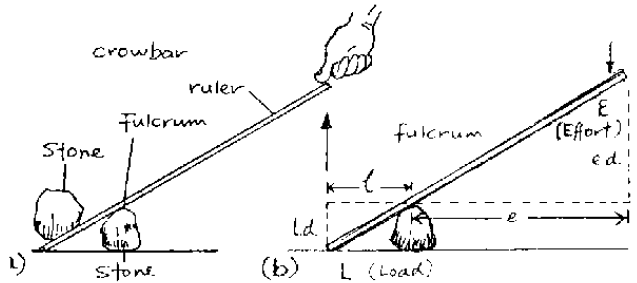
\includegraphics[width=0.49\textwidth]{./img/source/ruler-lever.png}
\end{center}

\begin{description*}
%\item[Subtopic:]{}
\item[Materials:]{Ruler, stones}
%\item[Setup:]{}
\item[Procedure:]{Make a lever using a ruler and a stone. Use it to lift a heavy stone or brick.}
%\item[Hazards:]{}
%\item[Questions:]{}
%\item[Observations:]{}
\item[Theory:]{The mechanical advantage is greater than one, i.e. the effort is less than the load; but the velocity ratio is greater than one, i.e. the effort distance is greater than the load distance.}
\item[Applications:]{Seesaw, pliers, wheelbarrow, bottle opener, forearm, etc.}
\item[Notes:]{Now slide the ruler down so that the fulcrum is near the center and try to lift the stone. Is it easier or more difficult?}
\end{description*}

\vfill
\columnbreak

\subsection{Uses of Levers}

\begin{center}
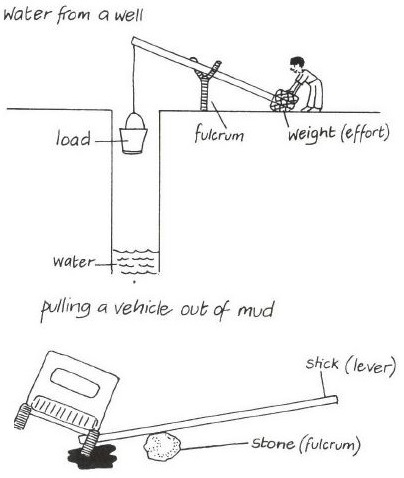
\includegraphics[width=0.49\textwidth]{./img/vso/using-levers.jpg}
\end{center}

\begin{description*}
%\item[Subtopic:]{}
%\item[Materials:]{}
%\item[Setup:]{}
%\item[Procedure:]{}
%\item[Hazards:]{}
%\item[Questions:]{}
%\item[Observations:]{}
%\item[Theory:]{}
\item[Applications:]{Levers can reduce the work needed to move loads.
Ask students where levers are used in their own communities.}
%\item[Notes:]{}
\end{description*}

\subsection{The Seesaw}

\begin{center}
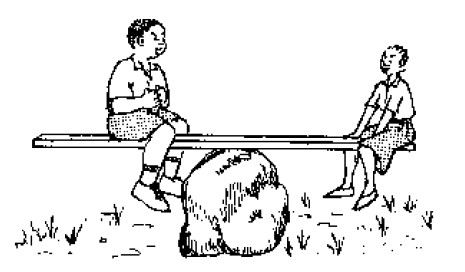
\includegraphics[width=0.4\textwidth]{./img/source/mechanics.png}
\end{center}

\begin{description*}
%\item[Subtopic:]{}
%\item[Materials:]{}
%\item[Setup:]{}
%\item[Procedure:]{}
%\item[Hazards:]{}
%\item[Questions:]{}
%\item[Observations:]{}
%\item[Theory:]{}
\item[Applications:]{The seesaw, pliers, the wheelbarrow, tweezers, the bottle opener, the forearm, the roman
steelyard, etc. are all levers.}
%\item[Notes:]{}
\end{description*}

\columnbreak

%==================================================================================================%

\section*{Pulleys}


\subsection{Simple Pulleys}
\label{sub:pulleys}

\begin{center}
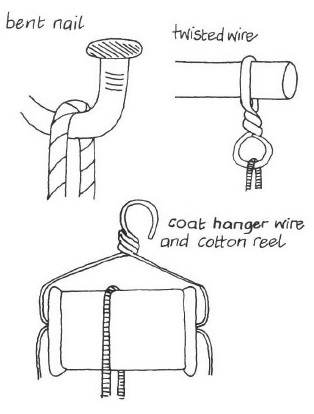
\includegraphics[width=0.45\textwidth]{./img/vso/pulleys.jpg}
\end{center}

\begin{description*}
%\item[Subtopic:]{}
\item[Materials:]{Nails, wire, coat hanger, water bottle, cotton reel}
%\item[Setup:]{}
\item[Procedure:]{Construct pulleys using any of the methods shown above. Alternatively, cut off the tops of water bottles just below the lip where the cap rests.}
%\item[Hazards:]{}
%\item[Questions:]{}
%\item[Observations:]{}
%\item[Theory:]{}
\item[Applications:]{Flagpole, well buckets, construction of tall buildings, etc.}
%\item[Notes:]{}
\end{description*}

\subsection{Uses of Pulleys}

\begin{center}
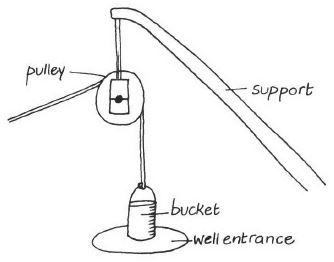
\includegraphics[width=0.4\textwidth]{./img/vso/uses-pulleys.jpg}
\end{center}

\begin{description*}
%\item[Subtopic:]{}
%\item[Materials:]{}
%\item[Setup:]{}
%\item[Procedure:]{}
%\item[Hazards:]{}
%\item[Questions:]{}
%\item[Observations:]{}
%\item[Theory:]{}
\item[Applications:]{Ask students where they have
seen pulleys used and why they
reduce the work of lifting loads.}
%\item[Notes:]{}
\end{description*}

\subsection{Single Pulley}

\begin{center}
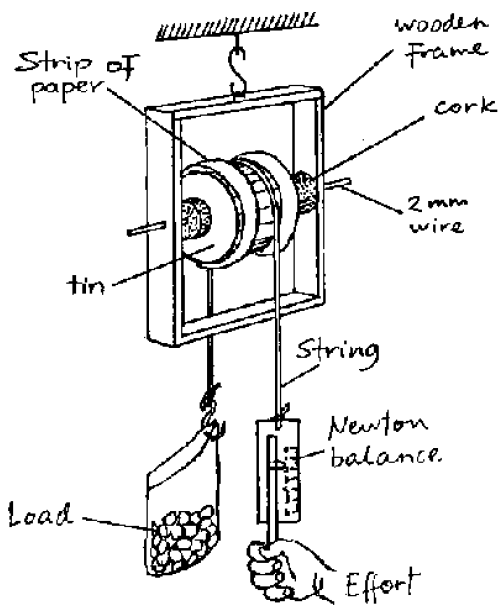
\includegraphics[width=0.45\textwidth]{./img/source/single-pulley.png}
\end{center}

\begin{description*}
%\item[Subtopic:]{}
\item[Materials:]{\nameref{sec:spring-balance}, bag of stones, string, stiff wire, thin wood, tin, cork, paper}
\item[Setup:]{Use one of the pulleys above, or construct one by poking holes on either end of a tin and placing a wire as an axle. Fix the axle into a wooden frame as shown.}
\item[Procedure:]{Attach a string to a load much heavier than the pulley (e.g. bag of stones). First measure the weight of the load using a spring balance. Then run the string across the pulley and record the effort required to lift the load.}
%\item[Hazards:]{}
%\item[Questions:]{}
\item[Observations:]{The weight of the load and the effort force required to raise it are equal.}
\item[Theory:]{A pulley has a M.A. of 1, meaning the load and effort are the same. The advantage of a single pulley is that it \emph{changes the direction} of the load. It is much easier to lift a heavy load by pulling downwards (with the help of your own weight) than by pulling upwards.}
%\item[Applications:]{}
%\item[Notes:]{}
\end{description*}

\vfill
\columnbreak

\subsection{Block and Tackle System}

\begin{center}
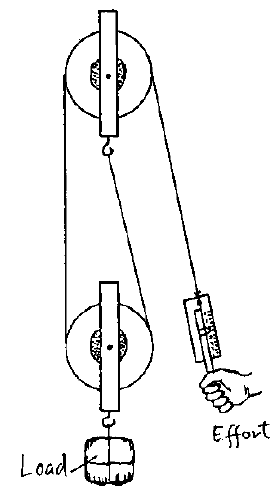
\includegraphics[width=0.35\textwidth]{./img/source/pulley-system.png}
\end{center}

\begin{description*}
%\item[Subtopic:]{}
\item[Materials:]{2 pulleys, string, \nameref{sec:spring-balance}, load (bag of stones)}
\item[Setup:]{Connect two single pulleys as shown in the figure, using any of the designs described above.}
\item[Procedure:]{Use this system to lift the same load as in the previous activity. Measure the effort using a spring balance.}
%\item[Hazards:]{}
%\item[Questions:]{}
\item[Observations:]{It is easier to lift the load this time, i.e. the effort is smaller.}
\item[Theory:]{Neglecting friction and the weight of the pulley, the M.A. will be 2, i.e. the load is twice the effort. The V.R. is equal to the number of pulleys in the system, in this case 2.}
%\item[Applications:]{}
\item[Notes:]{Try with more pulleys and see how it affects the M.A.}
\end{description*}

\vfill
\columnbreak

\subsection{Strength vs. Science}

\begin{center}
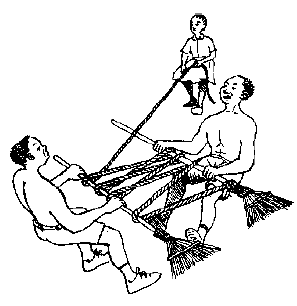
\includegraphics[width=0.45\textwidth]{./img/source/pulley-strength.png}
\end{center}

\begin{description*}
%\item[Subtopic:]{}
\item[Materials:]{2 broomsticks/jembe sticks, rope}
%\item[Setup:]{}
\item[Procedure:]{Fix one end of a rope to one stick and wind it back and forth around the two sticks as shown. Have 2 strong students pull on the sticks and one small student pull the other end of the rope.}
%\item[Hazards:]{}
%\item[Questions:]{}
\item[Observations:]{The small student wins.}
\item[Theory:]{This is an arrangement of ``broomstick pulleys.'' The small student requires much less effort to pull the heavy loads of the two strong students. However, the small student will have to move farther than the others.}
%\item[Applications:]{}
%\item[Notes:]{}
\end{description*}

\vfill
\columnbreak

%==================================================================================================%

\section*{Inclined Plane}


\subsection{The Ramp}

\begin{center}
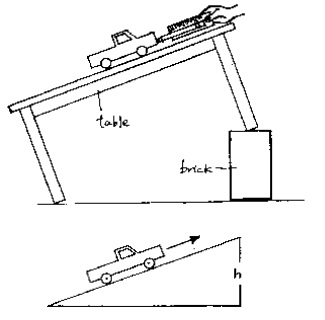
\includegraphics[width=0.4\textwidth]{./img/source/inclined-plane-2.jpg}
\end{center}

\begin{description*}
%\item[Subtopic:]{}
\item[Materials:]{Table, brick/books, \nameref{sec:spring-balance}, small weights/toy car}
%\item[Setup:]{}
\item[Procedure:]{Tilt a table by placing a brick or stack of books underneath its legs on one side. Weigh a small object (i.e. toy car) using a spring balance. Now pull the object up the tilted table and measure the effort with the spring balance.}
%\item[Hazards:]{}
%\item[Questions:]{}
\item[Observations:]{The effort is smaller than the load (weight of the object).}
\item[Theory:]{The effort distance is the distance moved along the table, whereas the load distance is the \emph{vertical} distance that the object moves. Thus, both the M.A. and V.R. depend on the angle of inclination of the plane.}
\item[Applications:]{Hills, ramps, screws, Egyptian pyramids}
%\item[Notes:]{}
\end{description*}

%==================================================================================================%

\section*{Wheel and Axle}


\subsection{Bottle Cap Gearworks}

%\begin{center}
%\includegraphics[width=0.4\textwidth]{./img/source/.png}
%\end{center}

\begin{description*}
%\item[Subtopic:]{}
\item[Materials:]{Soda bottle caps, nails, small piece of wood}
%\item[Setup:]{}
\item[Procedure:]{Find the exact center of each bottle cap and poke a hole through it for the nail. Nail the caps into the wood at even intervals so that they can freely rotate and in turn cause others to rotate. Make different configurations and note the direction of rotation from one gear to another.}
%\item[Hazards:]{}
%\item[Questions:]{}
\item[Observations:]{Adjacent gears turn in opposite directions.}
\item[Theory:]{Gears allow for the direction of rotation of a force to be changed. If the gears are of different sizes, then the rates of rotation will also vary.}
%\item[Applications:]{}
%\item[Notes:]{}
\end{description*}

\vfill
\columnbreak

%==================================================================================================%

\section*{Hydraulic Press}

%See activities in the Form I topic of \nameref{sec:pressure}.

\subsection{Syringe Hydraulics}

\begin{center}
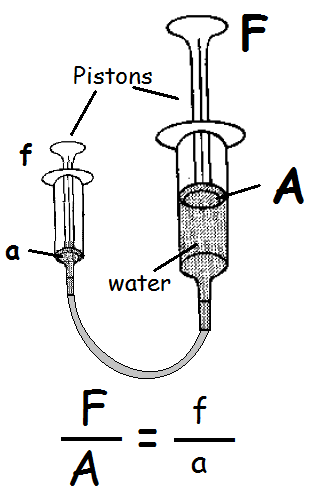
\includegraphics[width=0.3\textwidth]{./img/source/hydraulic-press.png}
\end{center}

\begin{description*}
%\item[Subtopic:]{}
\item[Materials:]{2 syringes of different size (5 mL and 20 mL), \nameref{sec:delivery-tube}, water}
%\item[Setup:]{}
\item[Procedure:]{Fill the larger syringe with water and attach one end of the rubber tubing to its end. Attach the other end of the tubing to the smaller syringe (with its plunger inserted all the way).}
%\item[Hazards:]{}
%\item[Questions:]{}
\item[Observations:]{Pushing the plunger of the larger syringe will cause the plunger of the smaller syringe to go out, and vice-versa.}
\item[Theory:]{When the effort piston is forced downwards, the pressure of the liquid, e.g. oil, is transmitted
equally in all directions in the whole liquid.
Therefore, the pressure at the load piston is the same as at the effort piston. Yet,
since the area of the load piston is greater than that of the effort
piston, the force at the load piston is greater than that at the effort piston. Thus, a small effort
will raise a big bad. However, the distance moved by the effort will be larger than that moved
by the load.}
\item[Applications:]{Hydraulic systems are used in brakes, pressing bales of cotton, lifting heavy loads (e.g.
vehicles in garages), etc.}
%\item[Notes:]{}
\end{description*}



\end{multicols}

\pagebreak